\documentclass[tikz,border=10pt]{standalone}\usepackage{amsmath}\usepackage{tikz}\usetikzlibrary{arrows.meta,positioning}\begin{document}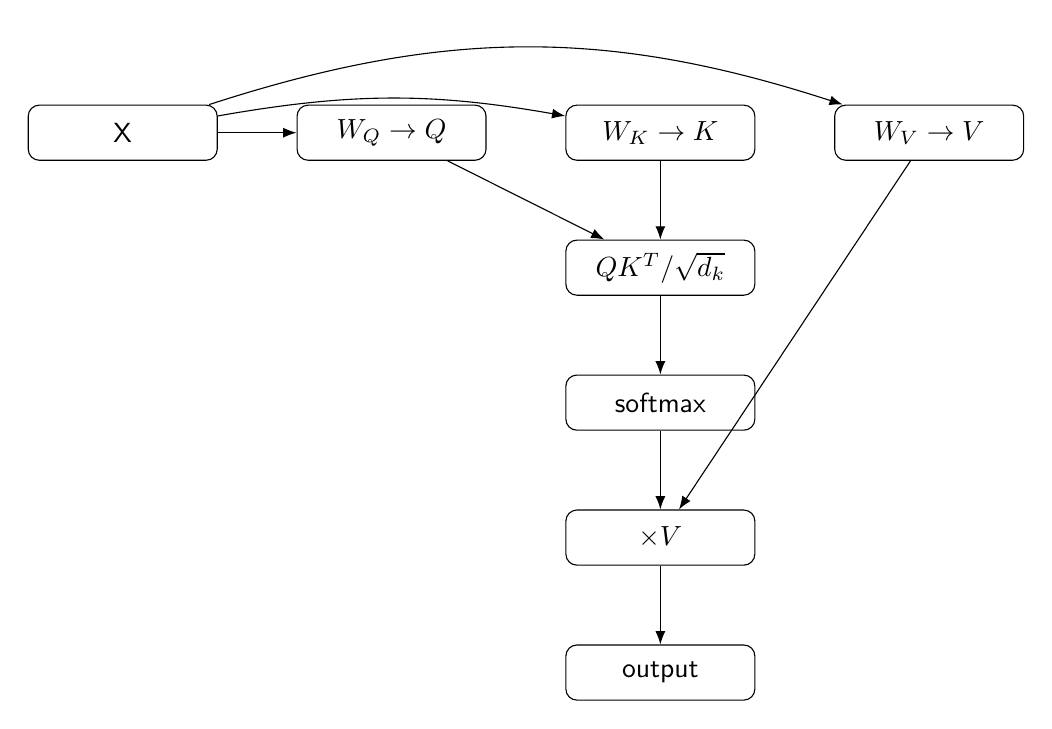
\begin{tikzpicture}[font=\sffamily,>=Latex,box/.style={draw,rounded corners,align=center,minimum width=2.4cm,minimum height=.7cm}]\node[box](x){X};\node[box,right=1cm of x](q){$W_Q\rightarrow Q$};\node[box,right=1cm of q](k){$W_K\rightarrow K$};\node[box,right=1cm of k](v){$W_V\rightarrow V$};\node[box,below=1cm of k](score){$QK^T/\sqrt{d_k}$};\node[box,below=1cm of score](sm){softmax};\node[box,below=1cm of sm](mul){$\times V$};\node[box,below=1cm of mul](out){output};\draw[->](x)--(q);\draw[->](x) to[bend left=10] (k);\draw[->](x) to[bend left=18] (v);\draw[->](q)--(score);\draw[->](k)--(score);\draw[->](score)--(sm);\draw[->](sm)--(mul);\draw[->](v)--(mul);\draw[->](mul)--(out);\end{tikzpicture}\end{document}
